%----------------------------------------------------------------------------------------------------------------------
\begin{frame}{Autodesk Inventor Sheet Metal has following features}

\begin{table}[!h]
\begin{tabular}[h]{@{}l l l l @{}}

\textcolor{yellow}{AliasFreeForm}	&
\textcolor{green}{Bend} &
\textcolor{green}{BendPart} &
\textcolor{blue}{Boss} \\

\textcolor{yellow}{BoundaryPatch} &
\textcolor{blue}{Chamfer} &
\textcolor{cyan}{CircularPattern} &
\textcolor{cyan}{Client} \\

\textcolor{blue}{Coil} &
\textcolor{blue}{Combine} &
\textcolor{green}{ContourFlange} &
\textcolor{green}{ContourRoll} \\

\textcolor{green}{CoreCavity} &
\textcolor{green}{CornerChamfer} &
\textcolor{green}{Corner} &
\textcolor{green}{CornerRound} \\

\textcolor{blue}{Cut} &
\textcolor{cyan}{Decal} &
\textcolor{blue}{Deleteface} &
\textcolor{blue}{Emboss} \\

\textcolor{yellow}{Extend} &
\textcolor{blue}{Extrude} &
\textcolor{blue}{FaceDraft} &
\textcolor{green}{Face} \\

\textcolor{blue}{FaceOffset} &
\textcolor{blue}{Fillet} &
\textcolor{green}{Flange} &
\textcolor{green}{Fold} \\

\textcolor{green}{Grill} &
\textcolor{green}{Hem} &
\textcolor{blue}{Hole} &
\textcolor{green}{Knit} \\

\textcolor{green}{Lip} &
\textcolor{green}{LoftedFlage} &
\textcolor{blue}{Loft} &
\textcolor{yellow}{Midsurface} \\

\textcolor{cyan}{Mirror} &
\textcolor{blue}{MoveFace} &
\textcolor{cyan}{Move} &
\textcolor{cyan}{NonParametricBase} \\

\textcolor{green}{PunchTool} &
\textcolor{cyan}{RectangularPattern} &
\textcolor{green}{Refold} &
\textcolor{blue}{ReplaceFace} \\

\textcolor{green}{Rest} &
\textcolor{blue}{Revolve} &
\textcolor{green}{Rib} &
\textcolor{green}{Rip} \\

\textcolor{blue}{RuleFillet} &
\textcolor{blue}{Sculpt} &
\textcolor{blue}{Shell} &
\textcolor{green}{SnapFit} \\

\textcolor{cyan}{Split} &
\textcolor{blue}{Sweep} &
\textcolor{yellow}{Thicken} &
\textcolor{blue}{Thread} \\

&\textcolor{cyan}{Trim} &
\textcolor{green}{Unfold} &\\
\\
\textcolor{yellow}{Surface} &
\textcolor{blue}{Solid} &
\textcolor{green}{SheetMetal} &
\textcolor{cyan}{Others}\\

\end{tabular}
\end{table}
%----------------------------------------------------------------------------------------------------------------------

\end{frame}

\begin{frame}{Thin Wall Part Features Taxonomy}
\vspace{0.1cm}
%\centering 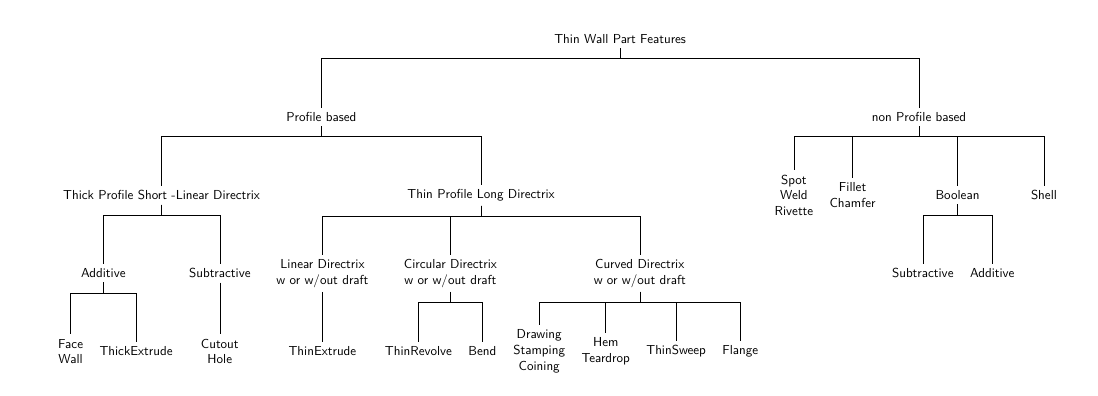
\includegraphics[width=\linewidth] {../Common/images/ThinWallFeaturesTaxonomy.png}
\resizebox{\linewidth}{!}{%
\begin{tikzpicture}
\tikzset{grow'=down}
%\tikzset{every tree node/.style={font=\small}}
\tikzset{every tree node/.style={align=center}}
\tikzset{sibling distance=6pt}
\tikzset{level distance=60pt}
\tikzset{edge from parent/.style=
{draw, edge from parent path={(\tikzparentnode.south) -- +(0,-8pt) -| (\tikzchildnode)}}, blank/.style={draw=none}}

%\Tree [.S 
%		[.NP 
%			[.Det 
%				the 
%			] 
%			[.N 
%				cat 
%			] 
%		]
%		[.VP 
%			[.V sat ]
%			[.PP 
%				[.P on ]
%				[.NP 
%					[.Det the ] 
%					[.N mat ] 
%				] 
%			] 
%		] 
%	]


\node{\Tree [.{Thin Wall Part Features}
		[.{non Profile based} 
			Shell
			[.Boolean Additive Subtractive
			]
			{Fillet\\ Chamfer}
			{Spot\\ Weld\\ Rivette}
		]
		[.{Profile based} 
			[.{Thin Profile Long Directrix}
				[.{Curved Directrix\\ w or w/out draft} Flange ThinSweep {Hem\\ Teardrop} {Drawing\\ Stamping\\ Coining} ]
				[.{Circular Directrix\\ w or w/out draft} Bend ThinRevolve ] 
				[.{Linear Directrix\\ w or w/out draft} ThinExtrude ] 
			] 
			[.{Thick Profile Short -Linear Directrix}
				[.Subtractive {Cutout\\ Hole} ]
				[.Additive ThickExtrude {Face\\ Wall} ] 
			] 
		]
	]
};

\end{tikzpicture}
}
\end{frame}

